\documentclass[journal,onecolumn]{IEEEtran}
%\documentclass[draftcls,onecolumn]{IEEEtran}
\usepackage{cite}
% *** GRAPHICS RELATED PACKAGES ***
\usepackage[pdftex]{graphicx}
\usepackage{authblk}
\usepackage{booktabs}
\usepackage{xcolor}
\usepackage{listings}
\usepackage{tikz}
\usepackage{adjustbox}
\usepackage{tabularx}
\usepackage{array}
\usepackage{wasysym}
\usetikzlibrary{positioning, shapes.geometric, arrows.meta, calc}
\usepackage[utf8]{inputenc}
\usepackage[T1]{fontenc}

% Format: \definecolor{<name>}{<model>}{<color-spec>}
\definecolor{amber}{rgb}{1.0, 0.75, 0.0}
\definecolor{myBlue}{HTML}{1E88E5}

\usetikzlibrary{shapes.geometric, positioning, arrows.meta, calc}

%\graphicspath{{../pdf/}{../jpeg/}}
\DeclareGraphicsExtensions{.pdf,.jpeg,.png}

% *** PDF, URL AND HYPERLINK PACKAGES ***
\usepackage[hyphens]{url}
\usepackage[hidelinks]{hyperref}
% correct bad hyphenation here
\hyphenation{op-tical net-works semi-conduc-tor}

% \usepackage{draftwatermark}
% \SetWatermarkText{DRAFT}
% \SetWatermarkScale{1}

\usepackage{easyReview}

\lstset{
	frame=single,                          % Draw a box around the code
	breaklines=true,                       % Wrap long lines automatically
	basicstyle=\small\ttfamily,            % Monospace font matching IEEE sizes
	keywordstyle=\color{blue}\bfseries,    % Style for syntax keywords
	commentstyle=\color{gray}\itshape,     % Style for code comments
	stringstyle=\color{red},               % Style for text strings
	showstringspaces=false,                % Don't show visible space markers
	numbers=left,                          % Position of line numbers
	numberstyle=\tiny\color{gray},         % Style for line numbers
	stepnumber=1                           % Number every line
}


\begin{document}
\title{SoK: Recent Developments in Hardware-Assisted Control Flow Integrity}
\author{\IEEEauthorblockN{Haorong Xu}\\
		Guangzhou, China \\
        Pioneer Academics \\
		haorongxu09@gmail.com}
\maketitle

\begin{abstract}

Control-flow Integrity (CFI) is a fundamental defense against control-flow hijacking attacks. Since software-only defenses incur substantial performance overhead, hardware-assisted CFI is proposed to incorporate hardware support for enforcing the integrity of control-flow transfers with relatively low cost. This Systematization of Knowledge (SoK) reviews recent developments in hardware-assisted CFI since 2022 by following a PRISMA-guided methodology. The reviewed defenses are organized into three categories: forward-edge, backward-edge, and universal CFI. We analyze their security guarantees, performance evaluation, and feasibility. Our analysis finds that recent work increasingly seeks fine-grained control-flow protection while relying on relatively coarse-grained hardware primitives, creating a tradeoff between security precision and defense complexity. Backward-edge protection has converged on hardware-assisted shadow-stack mechanisms, while forward-edge and universal approaches continue to explore more flexible enforcement strategies. We also identify inconsistencies in evaluation methodologies and highlight the need for more uniform benchmarks and practical deployment studies. Finally, we discuss open challenges and directions for future hardware-assisted CFI research.

\end{abstract}
\begin{IEEEkeywords}
	Systematic Review, Code reuse attacks, control flow integrity, hardware-based CFI implementations.
\end{IEEEkeywords}

\section{Introduction}

\subsection{Motivation}

From January 1st, 2025 to August 10th, 2026, over 60 vulnerabilities have been reported on the Common Vulnerabilities and Exposures system that involve altering the control flow \cite{cve-website}. Despite decades of mitigation against memory corruption, control-flow hijacking remains a prevalent attack vector. Attackers continue to bypass basic defenses such as address-space layout randomization (ASLR). Attacks such as return-oriented programming (ROP), jump-oriented programming (JOP), and counterfeit object-oriented programming (COOP) give rise to control-flow integrity (CFI) protections.

CFI is a security policy that ``dictates the software execution must follow a path of a Control-Flow Graph (CFG)''\cite{Abadi05}. CFI solutions are either software-based, hardware-based, or hardware-assisted\cite{Kumar22}. Software-only solutions are penalized by severe performance overhead\cite{Kumar22}; hardware-only solutions are inherently less flexible due to their long design and manufacturing process, and they are also often coarse-grained and difficult to deploy. Therefore, hardware-assisted CFI attempts to move part of the protection mechanism into privileged hardware-supported components to secure the integrity of control-flow transfer while reducing the performance cost.

In this SoK, hardware-assisted CFI refers to a defense in which a hardware feature, such as processor extensions and hardware monitoring facilities, participates in enforcing or detecting control-flow anomalies, while software counterparts provide policy generation, instrumentation, or runtime coordination.

Recent works have introduced various hardware-assisted CFI, whose mechanisms and dependent hardware primitives differ substantially. However, since prior systemizations, such as the works by de Clerq et al.\cite{Clercq17}, predate newly released hardware primitives that enabled numerous novel CFI techniques. More recent works, including the review by Kumar et al.\cite{Kumar22} and \cite{Li23}, provide useful foundations but do not fully address the scope of this SoK. Kumar et al.'s work\cite{Kumar22} classifies CFI according to whether the protection is implemented at the binary, process, or system level. While it captures the deployment location, the categories do not describe the mechanisms of CFIs. Some recently proposed CFIs are also implemented at multiple levels, so a CFI can be classified into multiple categories. Li et al.\cite{Li23} instead organize CFI defenses according to their implementation strategies. This organization is informative but limited in providing unified comparisons. Given the limitations of existing surveys, a current systemization is therefore needed. In our work, we propose a novel taxonomy to aggregate CFIs into three groups: forward-edge protection, backward-edge protection, and universal protection.

In this SoK, we exclusively focus on CFIs against  traditional architectural control flow hijacking - that is, speculative control flow hijacking such as the Spectre family attacks \cite{Kocher19} and interrupt-flow hijacking are not considered. Data-only attacks are also not considered, as they do not compromise control flow integrity. We restrict the scope of systemization to CFIs that are proposed since 2022 and intended for general-purpose computing systems.

\subsection{Research Questions}	

Based on the outlined scope, our SoK aims to answer the following research questions:

\begin{itemize}
    \item RQ1: What hardware-assisted CFIs are proposed since 2022?
    \item RQ2: What are the security guarantees of proposed defenses, and what limitations arise?
    \item RQ3: What are the trade-offs made by them in terms of feasibility and performance overhead?
    \item RQ4: What open problems should be addressed in this field?
\end{itemize}

To answer the research questions, we make the following contributions:

\begin{itemize}
	\item We present and systemize hardware-assisted CFIs proposed from 2022 to 2026 in Section \ref{sec:body}, including 18 primary studies.
	\item We present a novel taxonomy that classifies CFIs across 3 categories to compare their functionalities in section \ref{sec:body}.
	\item We assess the runtime performance and supporting evaluation strategies used in the field by examining the benchmarking suites, detailed in section \ref{sec:cost} and \ref{sec:perf}.
	\item We derive open questions and recommendations for future research in section \ref{sec:conclusion}.
\end{itemize}

\section{Background}

\subsection{Control Flow Hijacking Attacks} \label{sec:bg-control-flow-hijacking}

Control flow hijacking commonly stems from memory corruption attacks. Through writing to unintended memory locations, the attacker modifies the code or control data to divert the control flow to attacker-injected code or attacker-controlled addresses via returning or indirect jumps\cite{Ammar24}. Consequently, the injected code fragment or certain gadget (a part fragment of existing code) is executed.

Control flow hijacking is an umbrella term for several attacks. Due to its broad coverage, it is often discussed along with other attacks enabled by memory corruption, such as code injection attacks. To clearly define the scope of this review, the definition of control flow hijacking is given below.

According to Abadi et al.\cite{Abadi05}, the execution of programs is dictated by their \textit{Control Flow Graphs} (CFG), which show the intended path of control flow transfer. Any act that diverts the control flow from its intended path is considered a control flow hijacking. For example, the CFG for code in Listing \ref{list:example_cfg} is shown in Fig. \ref{fig:cfg-benign}.

\begin{lstlisting}[
	language=C, 
	frame=single, 
	captionpos=b,
	caption={Example code to demonstrate CFG}, 
	label={list:example_cfg}
	]
void baz();
void bar();
void foo(int arg)
{
    void (*func_ptr)() = &bar;
    if(arg == 1)
        baz();
    else
        func_ptr();
    ...
}
void main(int argc, char **argv)
{
    ...
    foo(argc);
    ...
}
\end{lstlisting}

\begin{figure}[!htb]
	\begin{minipage}{0.48\textwidth}
		\centering
		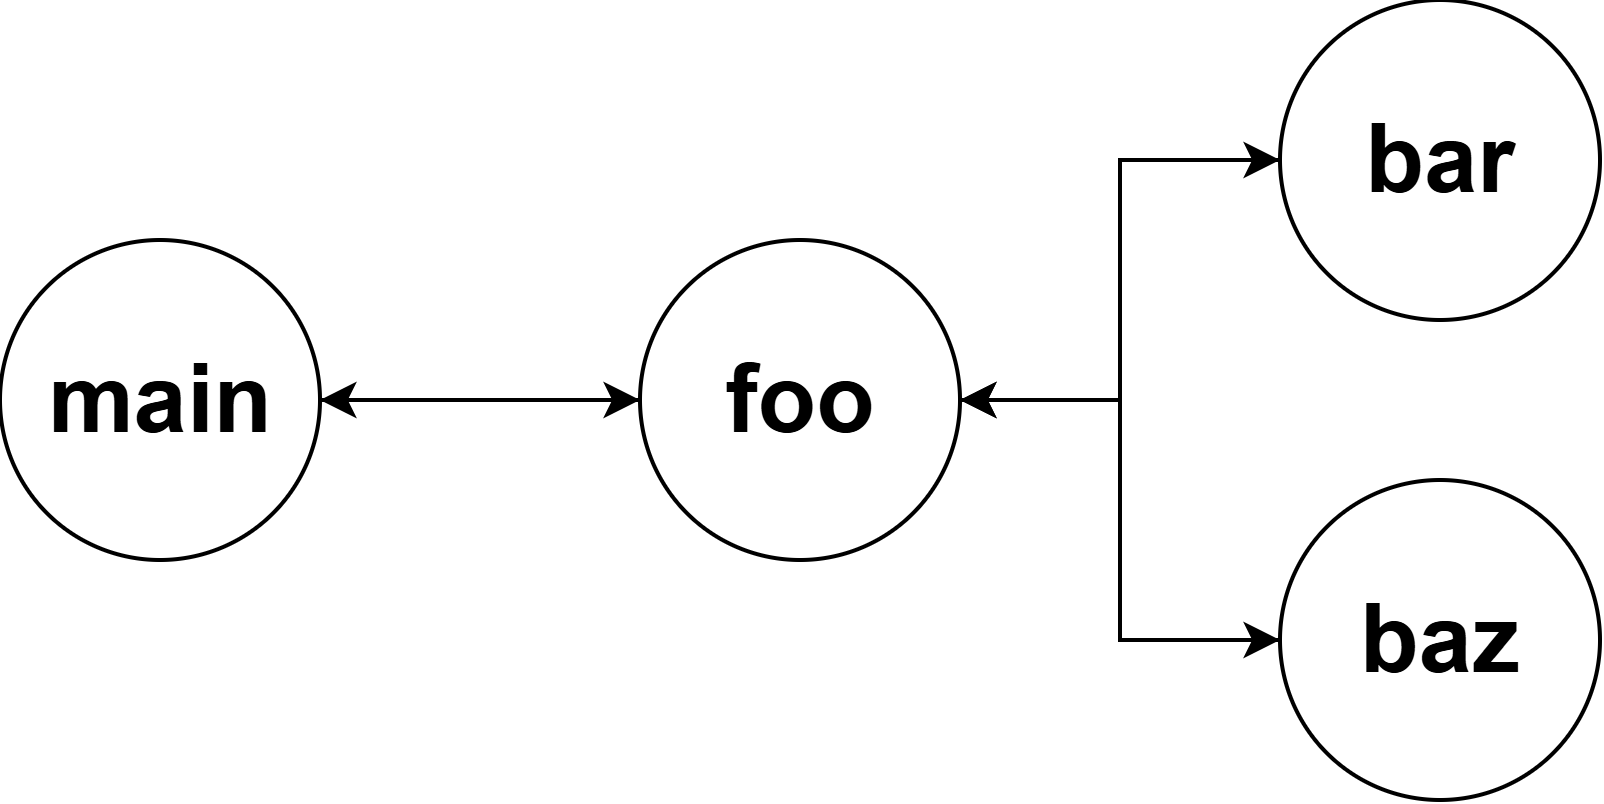
\includegraphics[width=\columnwidth]{cfg_benign.png}
		\caption{The control flow graph of code}\label{fig:cfg-benign}
	\end{minipage}\hfill
	\begin{minipage}{0.48\textwidth}
		\centering
		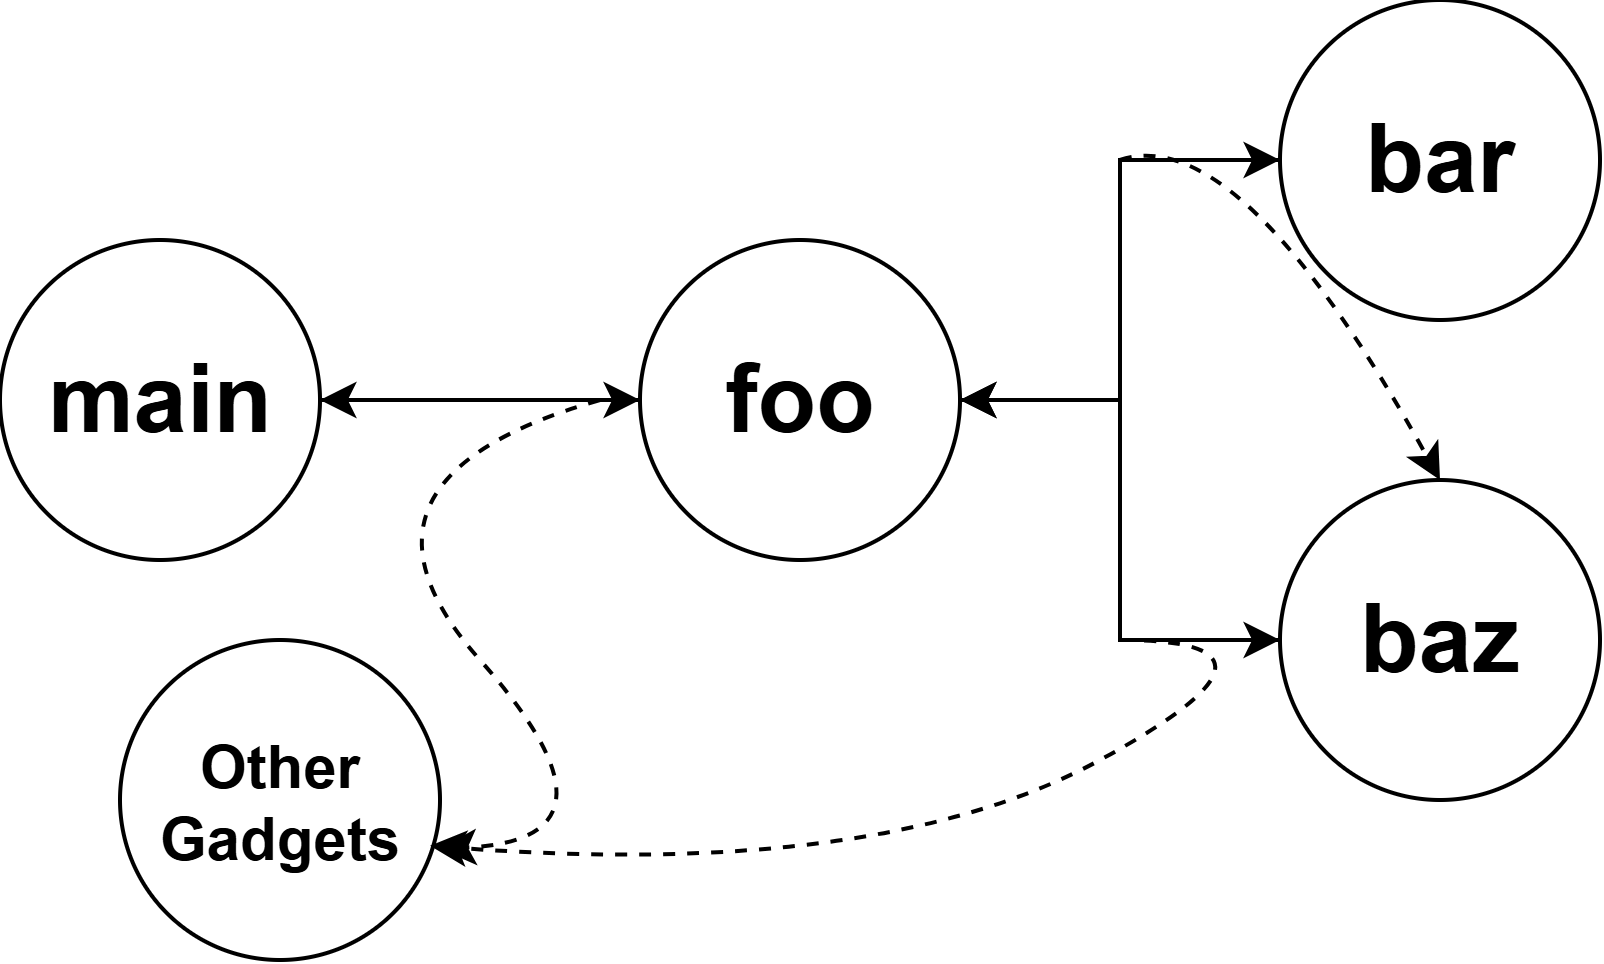
\includegraphics[width=\columnwidth]{cfg_attacks.png}
		\caption{Major types of control flow hijacking.}\label{fig:cfg-attacks}
	\end{minipage}
\end{figure}

The legitimate control-flow path would start from \texttt{main()} and proceed to \texttt{foo()}. \texttt{foo()} will call either \texttt{bar()} or \texttt{baz()}. Each function is represented by a node on the graph, while function calls are represented with forward arrows, or \textit{forward edges}. Then the control-flow returns from the functions in the reverse order in which they are called. Returning is represented with backward arrows, or \textit{backward edges}. Memory corruption attacks can modify several key items to divert the control-flow. These items are the attack surface of control-flow hijacking attacks, namely return addresses and function pointers. The attack vectors are described below:

\begin{figure}[!htb]
	\centering
	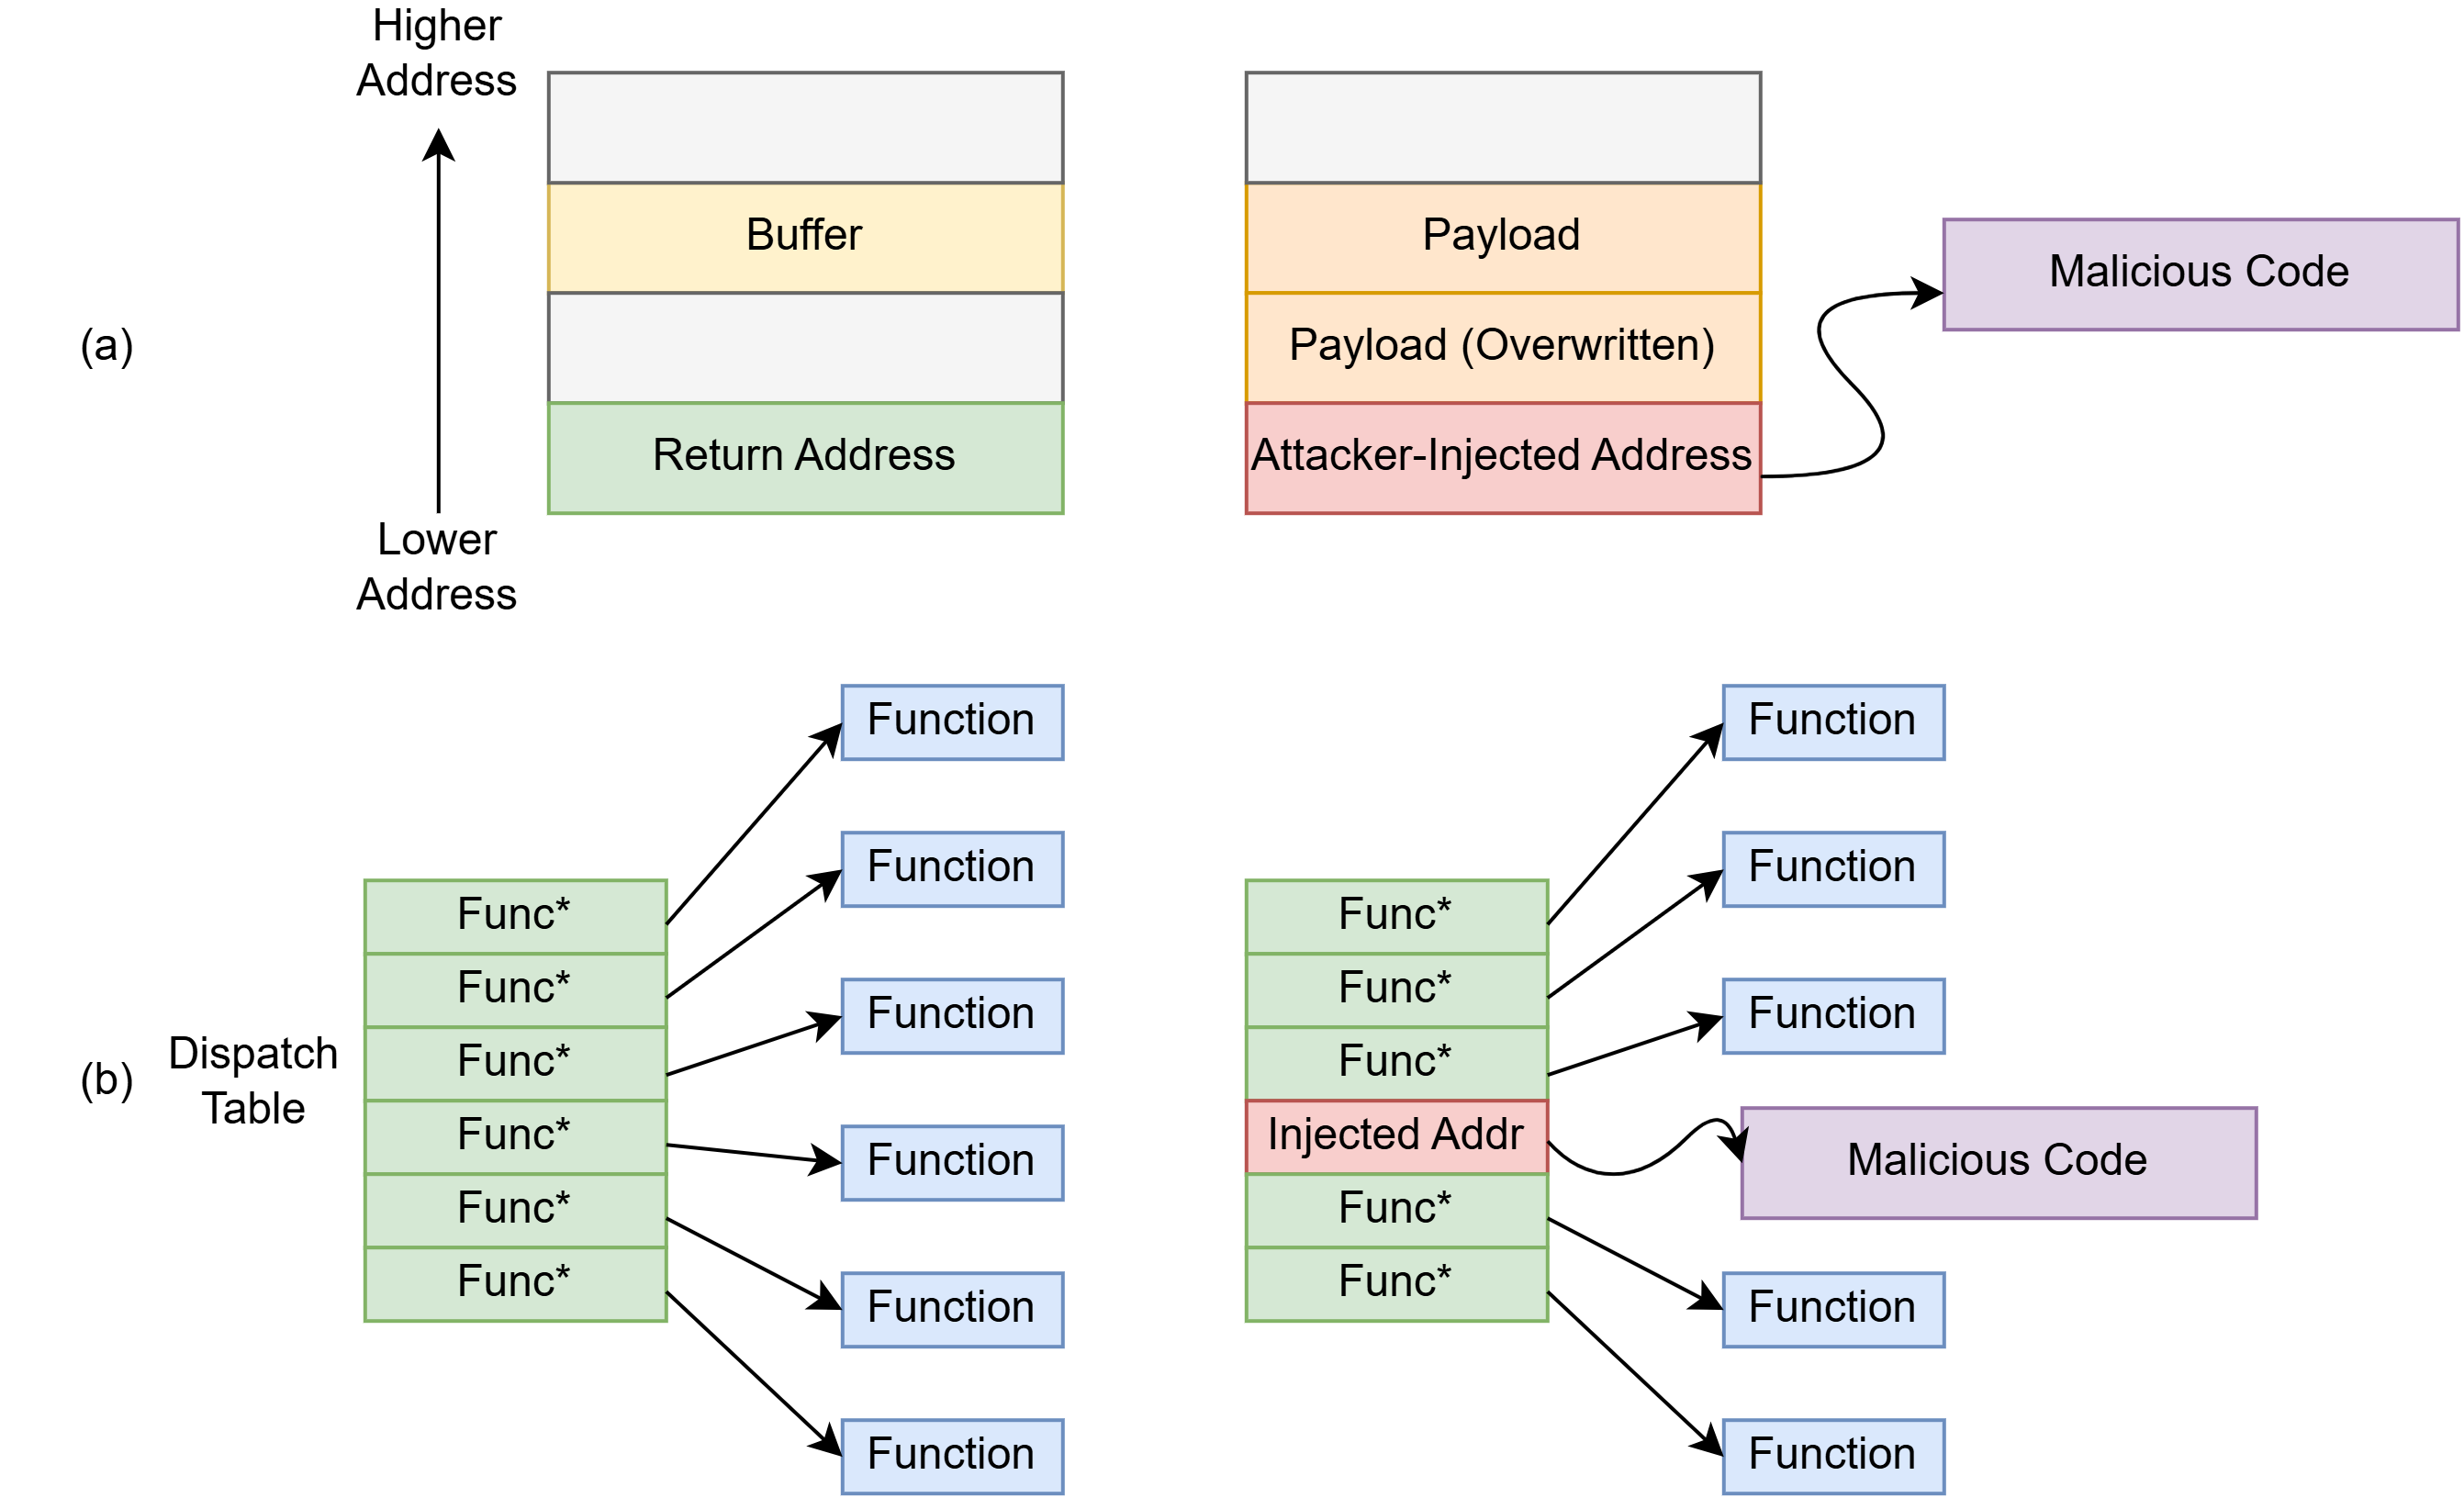
\includegraphics[width=\columnwidth]{attacks.png}
	\caption{Control-Flow Hijacking Attacks: ROP and JOP}\label{fig:attacks}
\end{figure}

\subsubsection{Return-Oriented Programming}

Return-oriented programming (ROP) hijacks the return address stored on the stack. A classic way to achieve this is via buffer overflow, illustrated in Fig. \ref{fig:attacks} (a). When an input string is copied to a buffer without a boundary check, the attacker can supply an input that is longer than the size of the buffer. The spilled part will overwrite the stack memory. By carefully calculating the memory address, the attacker can overwrite the return address stored on the stack, forcing it to point to an arbitrary address. When the control-flow returns from the function, it will jump to the attacker-injected address instead of its caller, thereby diverting the control flow. The impact on the control-flow graph is demonstrated in Fig. \ref{fig:cfg-attacks}: the backward edge is modified to point to other gadgets.

\subsubsection{Jump-Oriented Programming}

Jump-oriented programming (JOP) hijacks the function pointers in a dispatch table, which maps identifiers to certain functions. When a function pointer is used, instead of jumping to the legitimate target, the control-flow will instead be diverted to an attacker-supplied address. This is illustrated in Fig. \ref{fig:attacks} (b), and the impact on the CFG is shown in Fig. \ref{fig:cfg-attacks}: the forward edge is modified to point at an unintended gadget.

\subsubsection{Code Injection and Control-Flow Bending}

Code injection and control-flow bending attacks refer to two categories of control-flow hijacking attacks, depending on the destination of the diverted control-flow. If the control-flow is directed to attacker-injected code, the attack is classified as a code injection attack. In contrast, control-flow lands at an existing gadget in the code in a control-flow bending attack.

Defenses against memory corruption are widely deployed on modern systems, notably $W \oplus X$ memory. It ensures that a memory page can never be simultaneously writable and executable. Therefore, an exception will be raised when the attacker-injected code (writable page) is attempted to be executed. However, although $W\oplus X$ memory prevents attacker-injected code from being executed, it is not a CFI defense as it does not secure control-flow transfer: the control-flow is still diverted to the injected address.


\section{Methodology}

In this section, we introduce the two-stage systemization of knowledge process, which includes a) systematically reviewing defenses and b) systematizing hardware-assisted CFI. We follow the Preferred Reporting Items for Systematic
Reviews and Meta-Analyses (PRISMA) standard  for this work\cite{Page22} while only keeping the terms relevant to this study.

\subsection{Search Strategy}

The collection of sources consists of two phases: searching in digital databases and citation chasing. The digital databases used include ACM Digital Library (The ACM Full-Text Collection) \cite{ACMDLib}, IEEE Xplore \cite{IEEEXplore}, arXiv \cite{arXiv}, MDPI \cite{MDPI}, Springer Nature Link \cite{SpringerNature}, and ScienceDirect \cite{ScienceDirect} in conjunction with security publication venues including USENIX \cite{USENIX} and NDSS \cite{NDSS}. Since related studies are not fully indexed in these databases, Google Scholar \cite{GoogleScholar} is used for forward and backward citation chasing.

In the searching phase, we first created a list of keywords based on my experience and then extracted keywords from past CFI studies. The query string for each database derives from the keyword matrix and is adjusted to the constraints of their search engine. The final query strings are given in the Appendix (\ref{list:query} and \ref{list:arXiv_MDPI}). In addition, all searches are restricted to papers published in or after 2022, and all results were exported on the 31st of July, 2026.

\subsection{Screening Strategy}

To remove irrelevant studies from the search corpus, a three-phase screening process was carried out, including deduplication, title and abstract screening, and full-text screening. The following eligibility criteria are defined to specify studies to include: 

\begin{itemize} \label{list:criteria}
	\item EC1: The study must directly address defenses against control flow hijacking attacks. Defenses that are intended to prevent general memory corruption attacks should not be included.
	\item EC2: The study must either 1. propose a novel CFI defense or 2. evaluate a CFI defense.
	\item EC3: The CFI addressed in the study must be hardware-assisted. That is, it must be a hybrid method implemented at both hardware and software levels.
	\item EC4: The study must be published in or after 2022 and not reviewed already in \cite{Kumar22}.
	\item EC5: The study should be excluded if it is intended to defend against Spectre-like attacks which exploit speculative execution or interrupt-flow hijacking.
	\item EC6: The CFI proposed must be applicable to general computing devices instead of special-purpose devices such as embedded IoT devices.
	\item EC7: The defense proposed should not be solely intended to prevent non-control data attacks.
\end{itemize}

\subsection{Taxonomy}

In this work, we propose a novel taxonomy based on control flow transfer. As illustrated in Section \ref{sec:bg-control-flow-hijacking}, control flow hijacking can happen at either a forward-edge or a backward-edge. A forward-edge represents control flow being transferred from a caller to a target, or a callee, while a backward-edge represents returning from a callee to a caller, primarily returning from function calls. Based on the control flow edges that a hardware-assisted CFI protects, we classify CFI into 3 categories: \textit{forward-edge protection}, \textit{backward-edge protection}, and \textit{universal protection}.

Forward-edge protections enforce the integrity of forward control flow transfer, including indirect calls and jumps such as calling via function pointers and virtual function dispatching. This category of protections thereby prevents jump-oriented programming (JOP). The implementations of forward-edge protections mostly focus on securing function pointers.

Backward-edge protections protect against return-oriented programming (ROP), which tampers with the instruction that the program jumps to when returning from a function call, often to attacker-injected code or unintended gadgets. Backward-edge protections primarily achieve this goal by securing the return addresses stored on the stack, such as by creating a copy of return addresses (known as a shadow stack). This is not to be confused with protections against code injection attacks, which prevent malicious code from being written into memory or executed (such as W $\oplus$ X memory).

Universal protections refer to mechanisms that provide CFI enforcement on both forward and backward-edges. CFIs are only placed in this category if they guarantee security regardless of types of control flow transfer. 

As such, the taxonomy features mutually exclusive and comprehensive categories based on the security scope of the proposed CFI, rather than a specific implementation strategy.

\section{Results of the Search and Selection Process}

\begin{figure}[!htb]
	\centering
	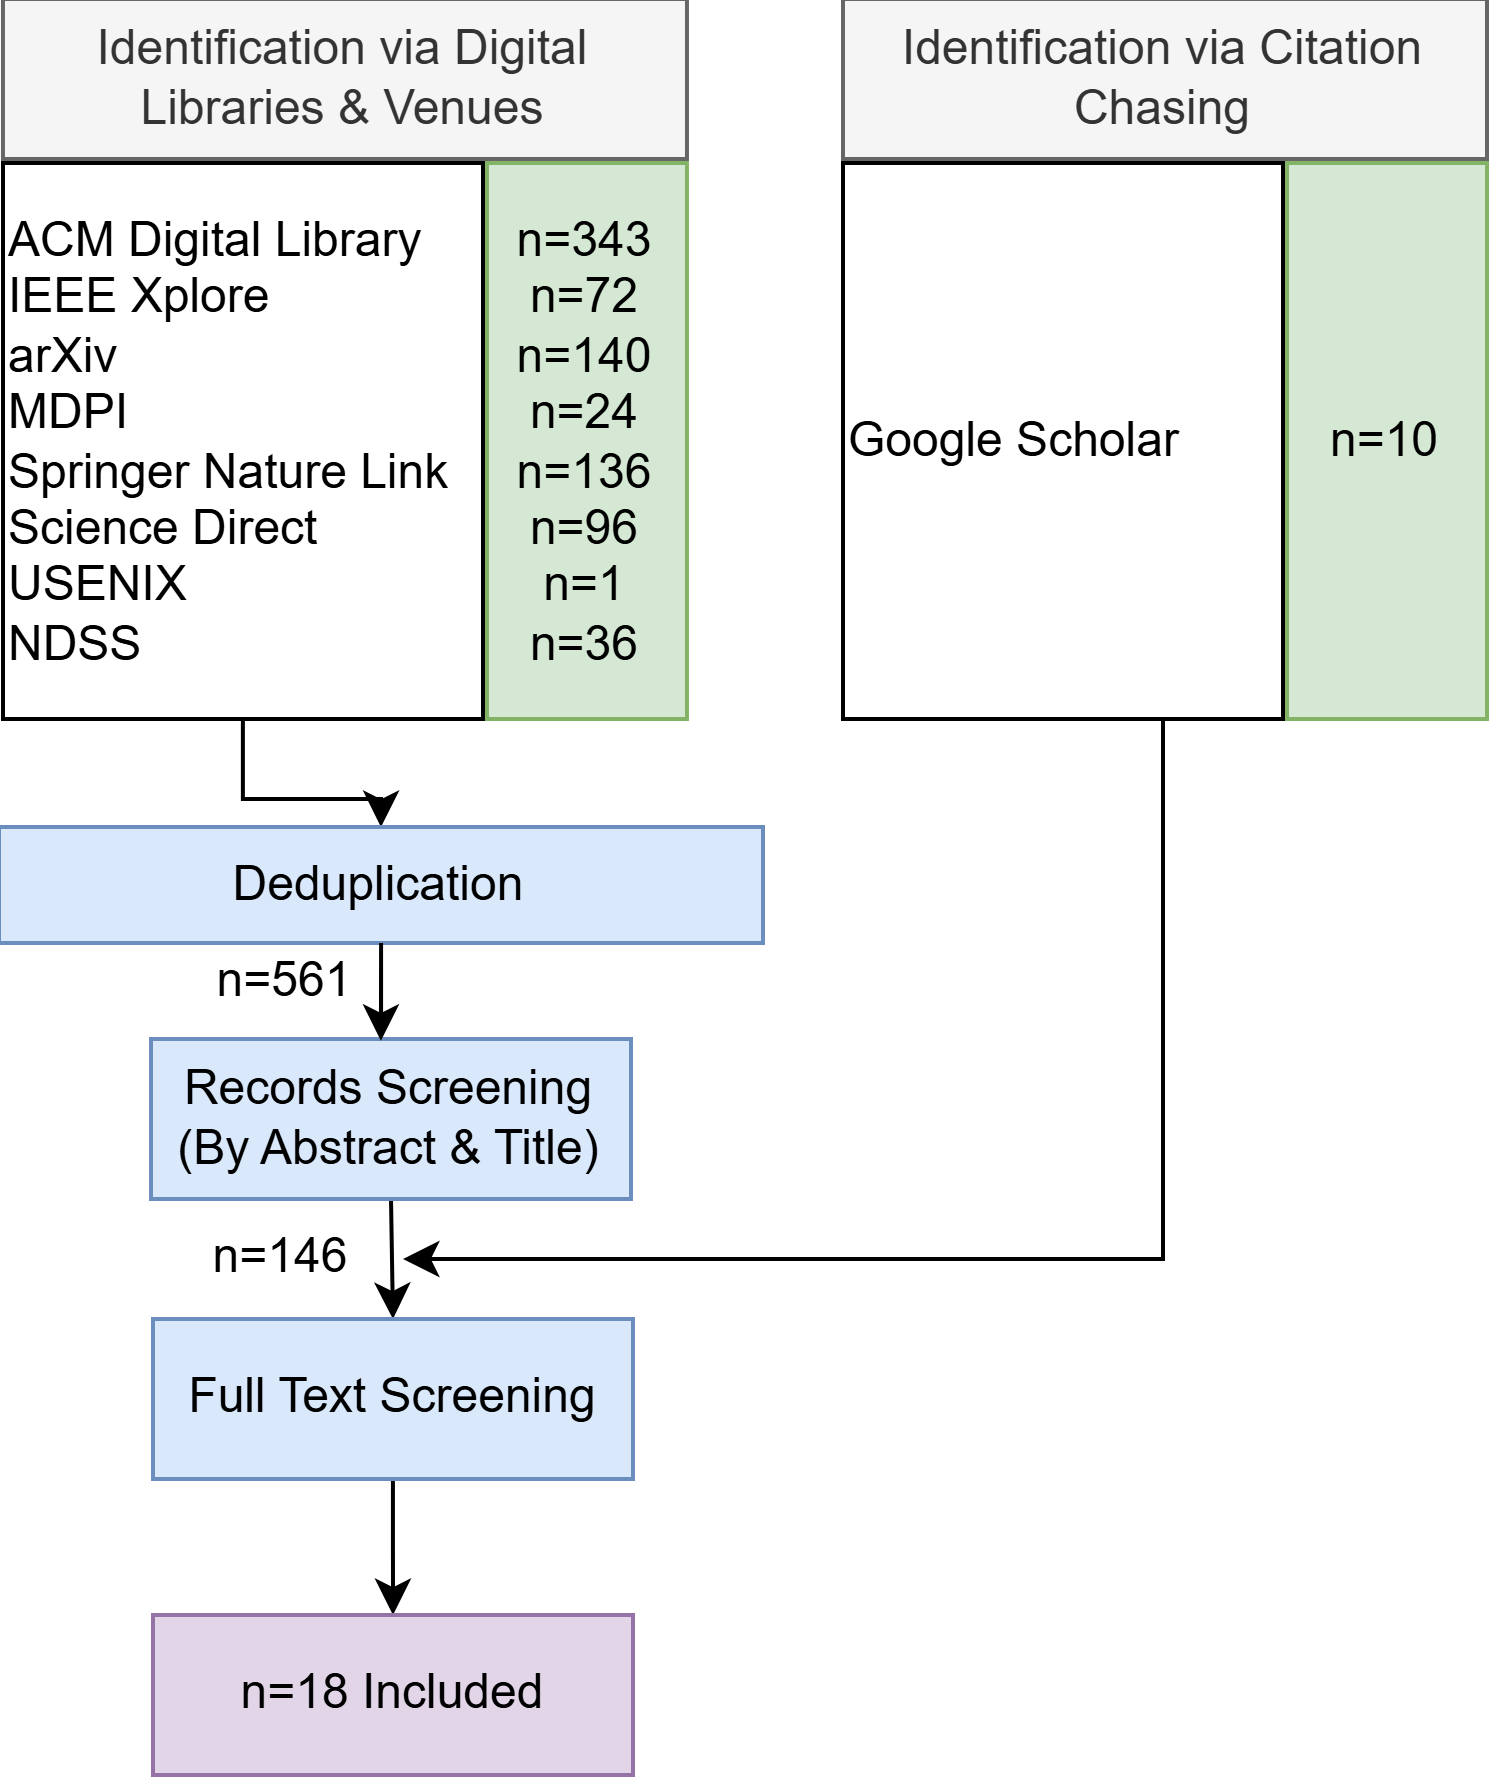
\includegraphics[width=0.5\columnwidth]{prisma.png}
	\caption{Adapted PRISMA flow chart}\label{fig:prisma}
\end{figure}

The search query presented in \ref{list:query} and \ref{list:arXiv_MDPI} yields 343 entries from ACM Digital Library, 72 from IEEE Xplore, 140 from arXiv, 24 from MDPI, 136 from Springer Nature Link, 96 from ScienceDirect, 1 from NDSS, and 36 from USENIX (868 entries in total). The deduplication process was carried out automatically by Zotero \cite{Zotero}, and 561 papers remained after removing identical items. The title and abstract screening involved checking for studies that were apparently inconsistent with the eligibility criteria, such as those that were not primarily focused on CFI. 146 papers remained after this phase, including studies whose relevance could not be determined by simply examining the title and abstract. After that, citation chasing was carried out using Google Scholar \cite{GoogleScholar} and Semantic Scholar \cite{SemanticScholar}. 10 papers were added as a result of citation chasing. The final screening process was conducted by reading the full text of all remaining studies, and 18 papers were selected to be included.

\section{Hardware-Assisted CFI}\label{sec:body}

\begin{table}[t]
	\centering
	\caption{Taxonomy of Hardware-Assisted CFI Defenses}
	\label{tab:cfi-taxonomy}
	\renewcommand{\arraystretch}{1.35}
	\setlength{\tabcolsep}{4pt}
	\begin{tabular}{
			>{\raggedright\arraybackslash}p{0.2\columnwidth}
			>{\raggedright\arraybackslash}p{0.35\columnwidth}
			>{\raggedright\arraybackslash}p{0.4\columnwidth}
		}
		\toprule
		\textbf{Category} &
		\textbf{Protected Transfer} &
		\textbf{CFI Paper} \\
		\midrule
		\textbf{Forward-edge} &
		Direct calls, indirect jumps (via function pointers), and virtual function dispatch &
		\cite{Demicco25}, \cite{Gaidis23}, \cite{Tan22}, \cite{Ismail24}, \cite{Yue25}, \cite{Kleftogiorgos26}, \cite{Zhao25b}, \cite{Hashemi26}, \cite{She24}, \cite{Unterguggenberger26}, \cite{Kim23} \\[2pt]
		
		\textbf{Backward-edge} &
		Returns &
		\cite{Moreira22}, \cite{Sharma25} \\[2pt]
		
		\textbf{Universal} &
		Forward- and backward-edge transfers &
		\cite{Zhao25}, \cite{Yeoh24}, \cite{Yoo22}, \cite{Zaidenberg26}, \cite{Sun26} \\
		\bottomrule
	\end{tabular}
\end{table}

The systematization has been carried out, and the results are shown in Table \ref{tab:cfi-taxonomy}. In this section, we analyze the security guarantees and functionalities of CFIs.

\subsection{Forward-Edge Protection} \label{sec:forward}

\begin{table}[t]
	\centering
	\caption{Comparison of Forward-Edge Protection CFI}
	\label{tab:forward-edge}
	\renewcommand{\arraystretch}{1.35}
	\setlength{\tabcolsep}{3.5pt}
	
	\begin{tabularx}{\columnwidth}{
			>{\raggedright\arraybackslash}p{0.15\columnwidth}
			>{\centering\arraybackslash}p{0.26\columnwidth}
			>{\raggedright\arraybackslash}X
		}
		\toprule
		\textbf{Paper} &
		\textbf{Granularity} &
		\textbf{Verification Mechanism} \\
		\midrule
		
		Intel CET (IBT)\cite{IntelIBT} &
		Coarse-grained &
		Landing Pad \\[2pt]
		
		ARM BTI \cite{ARMBTI} &
		Coarse-grained &
		Landing Pad\\[2pt]
		
		Zicflip \cite{RISCVInstructionSet} &
		Coarse-grained&
		Landing Pad\\[2pt]
		
		COGENT \cite{Demicco25} &
		Fine-grained &
		Tag matching based on equivalence classes \\[2pt]
		
		FineIBT \cite{Gaidis23} &
		Fine-grained &
		Tag matching between allowed callers and callees \\[2pt]
		
		ROLoad \cite{Tan22} &
		Fine-grained &
		Tag matching between allowed callers and callees \\[2pt]
		
		RSTI \cite{Ismail24} &
		Fine-grained &
		Check pointers integrity when loading into the memory, and tag matching based on equivalence classes\\[2pt]
		
		MOBIUS \cite{Yue25} &
		Fine-grained &
		Construct CFG by static and dynamic analysis. Use ARM BTI to trigger exception for checking at runtime \\[2pt]
		
		StreamCFI \cite{Kleftogiorgos26} &
		Fine-grained &
		Construct CFG by static analysis, and iterate it during execution. Use an external monitor to check indirect calls and virtual function dispatch at runtime \\[2pt]
		
		LeafHooks \cite{Zhao25b} &
		Fine-grained &
		Construct CFG by static analysis, and check for indirect jump targets against legitimate targets stored \\[2pt]
		
		SIC \cite{Hashemi26} &
		Fine-grained &
		Use static analysis to identify equivalence classes, and check for hashed function signatures at runtime \\[2pt]
		
		SCFI \cite{She24} &
		Fine-grained &
		Assign tags with static analysis, dividing functions into equivalence classes. Tags are checked at runtime. \\[2pt]
		
		Code Encryption with Intel TME-MK \cite{Unterguggenberger26} &
		Fine-grained &
		Source code encrypted with Intel TME-MK, and can only be decrypted at runtime by functions in the same equivalence class. \\[2pt]
		
		CPT \cite{Kim23} &
		Fine-grained &
		Construct CFG by static analysis and iterate during runtime. Checking handled by specialized hardware and instructions. \\[2pt]
		
		\bottomrule
	\end{tabularx}
\end{table}

Forward-edge protections are primarily used to prevent the control flow from being diverted by corrupted function pointers or virtual function dispatch tables. Forward-edge CFI is the most prevalent category of defenses among the three, mainly due to the coarse-grained nature of existing hardware primitive protections. The most widely adopted defenses are Intel Control-flow Enforcement Technology\cite{IntelIBT}, RISC-V Zicflip\cite{RISCVInstructionSet}, and ARM Branch Target Identification\cite{ARMBTI}. They are implemented as landing pads: legitimate targets for indirect branches (such as function pointer jumps) are marked with a special instruction. Upon a jump instruction, the processor checks if the target function starts with the padding instruction and raises an exception if not. While this approach prevents diverting the control-flow to arbitrary instructions, it cannot stop all control-flow bending attacks, since the gadget may also be a legal target. In response, many forward-edge protections seek to develop security policies to reduce the number of possible targets.

The majority of forward-edge CFIs employ a runtime verification approach: a possible CFG is generated before execution, by static or dynamic analysis, and all indirect jumps are validated against the CFG. Implementation strategies vary from tag-matching to code encryption, described as follows.

Tag-matching is a common approach to achieve this goal: it assigns the caller and legitimate callees a pair of matching tags that is verified upon an indirect jump. FineIBT\cite{Gaidis23}, COGENT \cite{Demicco25}, SIC \cite{Hashemi26}, and SCFI \cite{She24} are examples of tag-matching CFIs. They are all based on a static CFG generated during compilation, because they interleave tags and checking instructions into the binary of protected programs. The primary property that differentiates them is granularity: all of them assign tags based on equivalence classes. An equivalence class consists of all eligible indirect jump targets of a calling site, and all functions within the same equivalence class are eligible targets of each other. SCFI and COGENT are able to assign multiple tags to a function, so a function can be associated with multiple equivalence classes, while FineIBT and SIC only allow for one equivalence class per function. Consequently, more functions will be grouped into an equivalence class, reducing the precision of CFI policy\cite{Burow18}.

Other CFG validation methods include external monitoring and inlined checking. LeafHooks \cite{Zhao25b}, for example, embeds all allowed targets into the program's memory, and verification happens as inlined check nodes before indirect calls. MOBIUS \cite{Yue25} verifies control-flow transfer by leveraging ARM BTI. The binary is instrumented to execute a BTI instruction to trigger an exception, allowing a kernel module to check the control-flow transfer against the CFG generated by static analysis before it takes place. StreamCFI \cite{Kleftogiorgos26} uses a user-space counterpart to verify control-flow transfer: the program is instrumented to trigger the monitor to check the indirect call against a statically generated and dynamically iterated CFG asynchronously. CPT \cite{Kim23} features a similar approach that involves dynamically adjusting the CFG. It starts with a maximum possible CFG built during compilation, and marks edges as enabled when a function's address is assigned to a function pointer. Hence, only enabled edges on the CFG represent valid control-flow transfer. CPT verifies the forward edge prior to indirect jumps via a dedicated new hardware component, Edge Processing Unit (EPU).

A different approach to prevent forward-edge hijacking focuses on hardening function pointers, as they are the primary attack surface, such as validating function pointers to ensure they are not tampered with, including ROLoad \cite{Tan22} and RSTI \cite{Ismail24}. Generally, this group of CFIs seeks to ensure pointers point to the intended objects. ROLoad, implemented as a RISC-V ISA extension, protects function calls and virtual function dispatch by guaranteeing pointers are fetched from read-only memory. This prevents attackers from tampering with the pointer itself but does not ensure the target object's integrity. Therefore, it also requires matching keys in the pointer and the function, similar to the tagging approach introduced earlier. RSTI relies on ARM Pointer Authentication (ARM PA)\cite{ARMPA} as a hardware primitive, which assigns a cryptographic Pointer Authentication Code (PAC) to pointers and verifies it before use. However, ARM PA is coarse-grained since the key it uses is fixed, and valid pointers can substitute each other, as demonstrated in the study by Yoo et al. \cite{Yoo22b}, essentially grouping all indirect call targets in one equivalence class. Therefore, RSTI addresses this limitation by supplying a modifier to PA that encompasses semantic information such as type, scope, and permissions extracted from the source code, which is usually discarded in the process of compilation.

Finally, code encryption \cite{Unterguggenberger26} stands out as a distinct protection. It leverages Intel Total Memory Protection - Multiple Key (Intel TME-MK) \cite{IntelTMEMK} to encrypt the instructions of each function with a designated key, and functions can only be decrypted by matching calling sites that hold the correct key. Still, this approach requires determining equivalence classes during compilation so that functions within the same class can be assigned an identical key.

\subsection{Backward-Edge Protection}

\begin{table}[t]
	\centering
	\caption{Comparison of Backward-Edge Protection CFI}
	\label{tab:backward-edge}
	\renewcommand{\arraystretch}{1.35}
	\setlength{\tabcolsep}{3.5pt}
	
	\begin{tabularx}{\columnwidth}{
			>{\raggedright\arraybackslash}p{0.15\columnwidth}
			>{\centering\arraybackslash}p{0.25\columnwidth}
			>{\centering\arraybackslash}p{0.2\columnwidth}
			>{\centering\arraybackslash}p{0.2\columnwidth}
			>{\raggedright\arraybackslash}X
		}
		\toprule
		\textbf{Paper} &
		\textbf{Storage Location} &
		\textbf{Key Location} &
		\textbf{Overflow Handling} &
		\textbf{ISA Modification} \\
		\midrule
		
		Zicfiss \cite{RISCVInstructionSet} &
		Shadow Stack&
		N/A&
		No&
		RISC-V Standard ISA\\
		
		Return-Address Encryption \cite{Moreira22} &
		Stack&
		Supervisor&
		No need to&
		RISC-V Extension\\[2pt]
		
		Optimized RAS \cite{Sharma25} &
		Isolated Memory&
		N/A&
		Data movement triggered by RAS full signal&
		No, modification is invisible to ISA\\[2pt]
		
		RetTag \cite{Wang22} &
		Stack&
		Customized Coprocessor&
		No&
		RISC-V Extension\\[2pt]
		
		\bottomrule
	\end{tabularx}
\end{table}
Backward control-flow transfers can only happen through function returns, leaving return addresses stored on the stack as the primary attack surface. With the long history of countering ROP, backward-edge protections have been widely deployed in modern processors. The most prevalent approach is Shadow Stack, including Intel CET\cite{TechnicalLookIntel}, AMD Shadow Stack \cite{InfinityGuard}, ARM Guarded Control Stack\cite{ArmArchitectureReference}, and RISC-V Zicfiss \cite{RISCVInstructionSet}. These primitive protections maintain a separate compact stack that stores only the return addresses of each stack frame in a protected region. When a function executes a return instruction, the processor compares the return addresses stored in the two stacks to prevent ROP.

Due to the maturity of backward-edge protections, the number of new CFIs has been limited. Recent CFIs mainly focus on improving the storage paradigm of the standard shadow stack, which adds a consistent storage overhead. Return-address encryption proposed by Moreira et al. \cite{Moreira22} and RetTag \cite{Wang22} protect the return address itself stored on the stack instead of creating a copy of all addresses, while Sharma et al. \cite{Sharma25} seek to improve the flexibility of RISC-V's Return-Address Stack (RAS).

Return-address encryption employs an in-place signing approach that includes a binary instrumentation tool along with an ISA extension to store a signed hash value of the return address on the stack with a secret key only known to the hypervisor. RetTag utilizes the unused bits in the return address to store a PAC and extends the ISA of RISC-V to support the generation and verification of PAC. However, RetTag requires a custom coprocessor to handle relevant instructions to avoid slowdown. Therefore, these two approaches eliminate the storage overhead introduced by the shadow stack. Although all aforementioned backward-edge protections harden the return addresses, the trust boundary differs significantly: standard shadow stack relies on the processor to keep track of legitimate addresses; in-place signing moves key management and cryptographic algorithms to the hypervisor; RetTag leverages a dedicated coprocessor for this task. 

The final approach proposed by Sharma et al. is an extension of the RAS for RISC-V. The standard hardware RAS is intended for predicting return addresses, extended by Zicfiss into a shadow stack. The size of a RAS is small: although its size is not specified by the ISA, it can be easily overflowed by deep recursive calls\cite{Sharma26}. This would not be detrimental for optimization purposes, as the processor instead uses fallback mechanisms for address retrieval. However, it can be dangerous in security-critical applications. Therefore, the extension proposes copying return addresses to a dedicated memory area on demand to prevent overflow, thereby supporting CFI for deep recursive calls.

\subsection{Universal Protection}

\begin{table}[t]
	\centering
	\caption{Comparison of Universal CFI}
	\label{tab:universal}
	\renewcommand{\arraystretch}{1.35}
	\setlength{\tabcolsep}{3.5pt}
	
	\begin{tabularx}{\columnwidth}{
			>{\raggedright\arraybackslash}p{0.15\columnwidth}
			>{\centering\arraybackslash}p{0.3\columnwidth}
			>{\centering\arraybackslash}p{0.3\columnwidth}
			>{\raggedright\arraybackslash}X
		}
		\toprule
		\textbf{Paper} &
		\textbf{Enforcement Location} &
		\textbf{Static / Dynamic CFG} &
		\textbf{Hardware Primitive}\\
		\midrule
		
		LibIHT \cite{Zhao25} &
		Kernel + User Space Module&
		Dynamic&
		Intel IBT\\[2pt]
		
		sMVX \cite{Yeoh24} &
		In-process&
		N/A&
		Intel MPK\\[2pt]
		
		PAL \cite{Yoo22} &
		In-kernel&
		Static&
		ARM PA\\[2pt] 
		
		Hypervisor-based Binary Protection \cite{Zaidenberg26} &
		Hypervisor&
		Static&
		Intel LBR\\[2pt]
		
		Hamk \cite{Sun26} &
		Host OS&
		Static&
		Intel PMU \& LBR\\
		
		\bottomrule
	\end{tabularx}
\end{table}

Unlike forward-edge or backward-edge protections, universal protections seek to harden the control-flow integrity of the entire program, observing or intercepting all control-flow transfers. \ref{tab:universal} compares them in enforcement location and hardware primitive. Based on their purposes, universal protections can generally be classified as either CFG-violation detection mechanisms or control-flow enforcement.

\subsubsection{CFG-Violation Detection}

CFG-Violation detection does not stop control-flow hijacking by itself, but instead detects such hijacking and halts the process before damage occurs. Two major hardware primitives for this purpose are performance counters and branch tracing, such as the Intel Performance Monitoring Unit (PMU) and Intel Last Branch Record (LBR). Intel PMU is an in-processor hardware component that keeps track of architectural and microarchitectural events such as the number of indirect branches taken\cite{IntelPMU}. Intel LBR records fine-grained records of branches taken, including the source and target, in a ring buffer\cite{IntelLBR}. Since control-flow hijacking leads to a path different from the intended one, there will be a discrepancy in control-flow-related statistics, especially branch targets. Hamk \cite{Sun26}, Hypervisor-Based Monitor \cite{Zaidenberg26}, and LibIHT \cite{Zhao25} leverage this data to detect ongoing attacks. Hamk implements the checking software in the host OS of a virtual machine, while it is implemented in the hypervisor in Zaidenberg et al.'s work; the checking software retrieves the content in the LBR after a set number of branches by utilizing the interrupt generated by the PMU or instructions injected during binary instrumentation. These records are then compared to a static CFG generated from the source code. LibIHT leverages Intel LBR along with Intel Branch Tracing Store (BTS), which also holds branch records but with a far greater capacity than LBR. It reconstructs a runtime CFG from the branches taken and compares it to a pre-defined one to identify inconsistencies. However, it is worth noting that BTS introduces a significant slowdown\cite{intel2015realtime}, which undermines the feasibility of LibIHT in time-sensitive systems.

sMVX \cite{Yeoh24} identifies attacks in a different way: it uses Multi-Variant Execution (MVX) to replicate the process when executing sensitive parts, while each clone possesses a differently randomized address space. Since control-flow hijacking relies on predicting the address of the target gadget, it is expected that the attack would fail in some variants. Comparing the execution traces against each other, sMVX can identify disparity in control flow which signals an attack.

\subsubsection{Attack Prevention}

In most modern computing systems, backward-edge or forward-edge CFI are usually deployed simultaneously, so there is not a strong motivation to develop a full, end-to-end solution. The only CFI in this sub-category is PAL \cite{Yoo22}. Similar mechanisms are seen in forward-edge protections: it leverages ARM PA to sign function pointers at generation and verify them at use in the kernel. It also embeds fine-grained context-sensitive labels into the signature to bind a pointer to a specific function type or memory object. In addition, it signs the return address so that it provides comprehensive protection for all control-flow transfers.

\section{Discussion}

\subsection{Implementation Cost} \label{sec:cost}


A significant challenge for hardware-assisted CFIs is managing implementation cost. Currently, we identify three issues that could add to this cost: binary instrumentation, hardware modification, and runtime overhead.

Almost all protections embed additional metadata, usually implemented as tags and extra checking instructions, into the binary, a process referred to as binary instrumentation. Binary instrumentation is mostly carried out during compilation but can also be performed post-compilation. The compiler is suitable for this task, as it has semantic information, such as types of function pointers, that hardware lacks access to. Semantic information enables the compiler to include CFG-related data into the binary for hardware to check. However, for this purpose, applying CFIs that leverage binary instrumentation creates a need to recompile existing software. This constraint does not only apply to the CFIs proposed in the literature, but also to primitive defenses, as landing pads are also inserted into the program by the compiler. Intel CET IBT, for example,  requires the compiler to mark jump targets with the ENDBR instruction\cite{ControlflowEnforcementTechnology}. 

Backward-edge protections also need instrumentation. For instance, a program must be compiled with a special tag (fcf-protection=return)\cite{FCFProtection}. For a user-space program to run with shadow stack, the program itself, all libraries used by the program, and the kernel must all be compiled with the shadow stack feature.

As such, it might not be feasible in all cases to enable CFI support at the software level, especially for software that depends on legacy libraries. Since enabling CFI requires access to the source code, it is also infeasible for users to enable CFI features without developers' support. Low-level software that includes assembly code further exacerbates this situation, because compilers cannot infer control-flow information from it. Meanwhile, widely adopted CFIs, such as shadow stack support, are not enabled by default for Linux kernels. Using shadow stacks requires building the kernel with a special option, which potentially complicates the use of CFIs\cite{ControlflowEnforcementTechnology}. Therefore, most Linux distributions do not enable user-space shadow stacks by default, undermining the security of current systems. To illustrate, it was not until the 2\textsuperscript{nd} of July 2026 that a default system-wide shadow stack feature was proposed for Fedora\cite{F45ChangeProposal2026}, a prevalent Linux distribution\cite{FedoraLinux}.

Another concern is the feasibility of hardware modification. A significant number of defenses are based on extending the ISA, which necessitates changing the hardware to enable CFI. While modifying hardware does not inherently prevent CFI from being massively deployed, it generally takes a long period of time before such modifications can be implemented in processors. Existing systems will likely not benefit from them, since it takes significant time and effort to migrate systems to new CFI-enabled hardware.

Performance overhead introduced by CFIs is another factor that hinders their application. Although most hardware primitives introduce negligible slowdown (such as Intel CET and ARM PA), certain features, such as Intel BTS, cause significant slowdown that makes it infeasible for real systems. Intel BTS has been replaced by its modern successor, Intel Process Trace (Intel PT), to provide the same functionality with negligible performance impact\cite{IntelProcessorTrace}. However, the performance overhead of hardware-assisted CFIs is often not negligible. Table \ref{tab:overhead} compares the reported performance overhead of CFIs analyzed in the study. Although many CFIs have reported low overhead (<1\% slowdown, for example), it should be noted that the performance might not be consistent. For instance, the performance of forward-edge protections often worsens in applications with extensive use of function pointers. Finally, compatibility with other CFIs and software is currently under-explored. Since some CFIs make substantial modifications to the way that primitive hardware mechanisms work, it is unclear whether two CFIs can be paired together.

\begin{table}[t]
	\centering
	\caption{Reported Runtime Performance Overhead of CFIs Analyzed}
	\label{tab:overhead}
	\renewcommand{\arraystretch}{1.35}
	\setlength{\tabcolsep}{3.5pt}
	
	\begin{tabularx}{\columnwidth}{
			>{\raggedright\arraybackslash}p{0.25\columnwidth}
			>{\centering\arraybackslash}p{0.35\columnwidth}
			>{\raggedright\arraybackslash}X
		}
		\toprule
		\textbf{Paper} &
		\textbf{Reported Overhead}&
		\textbf{Benchmark Used (In Order of Respective Overhead)}\\
		\midrule
		
		LeafHooks \cite{Zhao25b} &
		3.2\% and 1.55\% &
		UnixBench, Phoronix\\[2pt]
		
		MOBIUS \cite{Yue25} &
		5.78\% &
		SPEC2006 \\[2pt]
		
		SCFI \cite{She24} &
		0.78\%&
		SPEC2006\\[2pt]
		
		CPT \cite{Kim23} &
		1.2\%&
		Average on SPEC2006 and SPEC2017\\[2pt]
		
		LibIHT \cite{Zhao25} &
		0.66\%&
		Customized benchmarks\\[2pt]
		
		PAL \cite{Yoo22} &
		1\%, 3-5\%&
		Apache, Linux perf\\[2pt]
		
		sMVX \cite{Yeoh24} &
		7\%, 266\%, 223\%&
		Customized Benchmark, Nginx, Lighttpd\\[2pt]
		
		RetTag \cite{Wang22} &
		0.11\%, 7.69\%&
		NBench, Coremark\\[2pt]
		
		ROLoad \cite{Tan22} &
		~0\%&
		SPEC2006\\[2pt]
		
		Return-Address Encryption \cite{Moreira22} &
		N/A&
		N/A\\[2pt]
		
		StreamCFI \cite{Kleftogiorgos26} &
		8.63\%&
		SPEC2017\\[2pt]
		
		RSTI \cite{Ismail24} &
		6.86\%-12.7\%, 5.36\%-21.47\%, 3.44\%-10.8\%, 3.93\%-12.76\% depending on security policy&
		SPEC2017, SPEC2006, PyTorch on CPython 3.9, Nginx\\[2pt]
		
		SIC \cite{Hashemi26} &
		1.7\%&
		SPEC2017\\[2pt]
		
		FineIBT \cite{Gaidis23} &
		0\%-1.94\%, 0\%-1.92\%, 1.17\%, 0.6\%, <0.5\%&
		SPEC2017, Nginx, Redis, MariaDB, SQLite\\[2pt]
		
		COGENT \cite{Demicco25} &
		0.94\%-5.24\%&
		SPEC2017\\[2pt]
		
		Hypervisor-based Binary Protection \cite{Zaidenberg26} &
		0.72\%, 2.4\%, 3.9\%&
		LMBench, OpenSSL, GZip\\[2pt]
		
		Code Encryption with Intel TME-MK \cite{Unterguggenberger26} &
		2.2\%-7.8\%&
		SPEC2017\\[2pt]
		
		Hamk \cite{Sun26} &
		1.7\%, 0.16\%, 1\% (average)&
		SPEC2006, LMBench, (cp, diff, tar -x, tar -c, make, sort, md5sum, dd, awk, OpenSSL)\\[2pt]
		
		RAS \cite{Sharma25} &
		2\%-14\%&
		CoreMark\\[2pt]
		
		\bottomrule
	\end{tabularx}
\end{table}

\subsection{Limitations of Performance Evaluation} \label{sec:perf}

Most studies presented in the systemization have carried out performance evaluation, and in many cases, substantial analysis, except for the Return-Address Encryption proposed by Moreira et al.\cite{Moreira22}. However, we notice three issues in the evaluation process: 1. inconsistent benchmarks are used in the literature, 2. outdated or unsuitable benchmarks, and 3. use of real-world applications as test cases is not universally adopted.

Most CFI evaluations, as illustrated in Table \ref{tab:overhead}, leverage different benchmarking tools, with the most widely used tool being SPEC CPU Benchmarks\cite{SPECCPUBenchmarks}. However, the field has yet to reach a consensus on the standard benchmark suite for CFI performance evaluation. Some studies instead rely on customized benchmarks and other testing suites such as UnixBench and LMBench. While using different benchmarks does not inherently undermine the validity of the study, it impedes cross-study comparisons.

The second issue arises from the benchmark suite itself. While SPEC is suitable for general-purpose benchmarking, it is not intended for evaluating the performance overhead of CFIs. The study of Xu et al.\cite{Xu19} shows that the complexity of the CFG of real-world software exceeds the scope of SPEC. Their quantitative evaluation suggests that many SPEC benchmarks have no strong correlation with CFI overheads in production software. Meanwhile, SPEC2006 is still used by some studies as the sole evaluation tool, while this benchmark suite was retired on the 8\textsuperscript{th} of January, 2018. At the time of writing, its successor, SPEC2017, used by most other studies, will also soon retire on the 11\textsuperscript{th} of November, 2026.  SPEC2026 was released on the 5\textsuperscript{th} of May, 2026, so it is understandable that none of the studies reviewed in this SoK had adopted it. Future studies, on the other hand, should use SPEC2026 to replace outdated tools to keep up with the latest industrial standard.

Lastly, the lack of real-world applications as testing tools raises our concerns. While a number of studies test performance with production software such as Nginx, an overwhelming majority of the studies selected rely purely on benchmarking suites. The performance impact across benchmark suites (such as SPEC) and real applications can exhibit a noticeable disparity, as shown in the case of sMVX \cite{Yeoh24} and Hypervisor-based Binary Protection \cite{Zaidenberg26}. In both cases, the overhead is significantly higher for real-world applications, which demonstrates the significance of such test cases.

Additionally, benchmarking with production software will benefit from a standardized approach. Different studies have used different software, including Nginx, OpenSSL, and PyTorch for evaluation. Nonetheless, the testing suite should consist of a variety of software that represents the performance impact of CFI in a production environment. For instance, the testing suite can include both heavyweight software (such as PostgreSQL and PyTorch) and lightweight components such as Nginx. Combining this software with desktop applications such as Chromium and Firefox will further ascertain the reliability of performance evaluation, such that the data obtained can be a good predictor of its overhead in various setups.

\subsection{Forward-Edge Protections: Retrofitting Hardware Primitives}

As shown in Table \ref{tab:forward-edge}, currently available hardware CFI primitives for forward-edge protections, including Intel CET, ARM BTI, and RISC-V Zicflip, are all designed for coarse-grained protection. They effectively stop hijacking the control flow to attacker-injected code or the middle of functions. However, since they are implemented as landing pads, they cannot differentiate between legitimate targets, so callers are not bound to any particular callees. Consequently, all the research seeks to retrofit coarse-grained CFIs to enforce fine-grained security policies.

Binary instrumentation, in most cases, is a by-product of this retrofitting process, which makes it ubiquitous in hardware-assisted CFIs. To leverage the hardware primitive while extending its functionality, CFIs have to implement checking mechanisms on top of hardware defenses and add new features to the hardware either by directly modifying its design or by implementing patches at the software level. As shown in Section \ref{sec:cost}, this leads to various problems associated with implementation cost. Notably, forward-edge protections are most affected by the disparity between fine-grained security policies and coarse-grained primitives, while backward-edge protections do not suffer from this issue. Instead, the shadow stack has become the standard approach that does not require further amendments to fit the security goals. Forward-edge protections, in contrast, do not have such an equivalent standard. ARM PA is the only primitive with built-in flexibility for supporting better granularity: it allows for 5 separate keys and a modifier (also known as context) that creates variation in the signature \cite{ARMPA}. Therefore, a great proportion of forward-edge defenses are designed for ARM architecture. To fundamentally change this situation, new hardware features must be developed for greater flexibility and granularity.

\subsection{Development of mitigations from 2022}

Backward-edge protection has been maturing since the introduction of Shadow Stack, which became the standard hardware primitive across different architectures, such as Intel's Control-flow Enforcement Technology (CET) \cite{ControlflowEnforcementTechnology}, AMD's Shadow Stack \cite{InfinityGuard}, and ARM's Guarded Control Stack (GCS) \cite{ArmArchitectureReference}. Recent research, therefore, mainly seeks to optimize the storage scheme, while leaving the design of shadow stack unchanged.

The landscape of forward-edge CFIs presents an opposite picture: the protections are fragmented into several categories. Currently, these categories primarily include tag-matching, code encryption, pointer hardening, and external monitoring. From the reported performance overhead in Table~\ref {tab:overhead}, none of them is in a significantly advantaged position compared with others. Finally, some protections, such as CPT\cite{Kim23}, completely discard available hardware primitives and propose new dedicated parts. Since each defense requires a different compiler toolchain and hardware setup, the field is yet to reach a consensus on the most effective protection.

Internally, forward-edge CFIs have also experienced a gradual transition from pure static analysis to dynamic analysis. As covered in Section \ref{sec:forward} and \ref{sec:cost}, forward-edge CFIs rely on precisely identifying the CFG to check for legitimate jump targets. However, static analysis necessarily generates an over-approximation of the actual CFG - there will be more edges (representing potential control-flow transfer) than there could possibly be, which undermines the effectiveness of CFI. Static analysis also struggles when the program extensively uses dynamic libraries and dynamically generated code, as the CFG of the dynamic code is not known in advance. In response, defenses have been increasingly adopting dynamic analysis to complement static analysis; examples include StreamCFI, MOBIUS, and CPT.

Finally, universal protections occupy the middle ground to oversee the entire CFG. However, some of them incur a high cost in deployment complexity, yet it offers no clear advantage over a combination of forward-edge protection with backward-edge primitive to justify this cost. For example, on the Intel x86 platform, enabling shadow stack along with FineIBT provides an efficient and comprehensive defense that weakens the necessity of a separate end-to-end solution.

\subsection{Limitations}

A primary limitation of this study arises from the inclusion and exclusion criteria presented in Section \ref{list:criteria}. They were designed to maintain a tight focus on recent hardware-assisted CFI against traditional control-flow hijacking attacks, but several criteria introduce limitations that diminish the generalizability of our observations.

Since EC2 excludes attack-related papers, our evaluation is mostly based on authors' self-reported security claims, which can lead to optimistic bias. Therefore, recent attacks that can undermine the effectiveness of CFIs are not addressed. Strict adherence to EC4 also narrows our vision to most recently published works, so long-term trends that span across decades cannot be identified.

EC5, EC6, and EC7 also restrict the scope of this study. EC5 rejects CFIs intended for Spectre-family microarchitectural attacks or interrupt-flow hijacking, which are an increasingly relevant category of CFI. EC6 effectively excludes papers on IoT devices that have produced distinct CFI mechanisms under resource constraints. Lastly, EC7 excludes data-only attacks. Though data-only attacks are not control-flow hijacking in the conventional sense, it affects the control-flow in practice. Such strict eligibility criteria also prevent us from analyzing whether current CFIs are sufficient in the continuously evolving attack landscape.

\section{Conclusion}

\subsection{Contributions And Synthesis} \label{sec:conclusion}

We systematically analyzed 18 hardware-assisted CFI defenses published between 2022 and 2026, adhering to a PRISMA-guided standard. Sources were collected across 8 digital libraries and publishing venues. We propose a novel taxonomy that classifies CFIs into three mutually exclusive categories: forward-edge protection, backward-edge protection, and universal protection. 11 CFIs are classified as forward-edge defenses, 2 as backward-edge defenses, and 5 as universal.

We find that forward-edge research takes up the most volume of existing CFIs, driven by retrofitting coarse-grained hardware primitives (such as Intel CET IBT, ARM BTI, RISC-V Zicflip) to accommodate fine-grained security policies. Backward-edge protections have reached a common ground on the shadow stack as the universal standard. Recent works focus on storage optimization rather than new schemes. In contrast, forward-edge protections are more fragmented, featuring multiple defense mechanisms.

Additionally, we identify major issues of evaluation practices: the benchmarking suites used are inconsistent across studies; some tools are not suitable or outdated; there is a lack of real-world applications; there is not a standardized basket of production software for testing.

\subsection{Future Outlook}

The analysis in the Discussion has pointed to several directions for future research. First, further research is needed to address the generation of CFG, as static analysis is incapable of dealing with dynamic code. Second, the research community needs to develop a benchmark suite that comprehensively measures overheads introduced by CFI, along with testing performance impact on real-world software. Third, further work is needed to investigate the effect of combining CFIs to yield comprehensive protection. Finally, the field should invest in CFI abstraction that can be mapped to hardware primitives on different platforms, such as Intel CET IBT, ARM PA, and ARM BTI, which will unify the field that is currently fragmented by architectures.

\section*{Acknowledgment}

I would like to express my very great appreciation to Prof. Hanan Hibshi for her valuable and constructive suggestions during the planning and development of this research work. Her willingness to give her time so generously has been very much appreciated.

I would also like to extend my thanks to the scholars and staff members of Pioneer Academics for their encouragement and kindness in offering me constructive advice during the research.

Finally, I wish to thank my parents and friends for their support throughout my research.

I acknowledge the use of Grammarly (\url{https://www.grammarly.com/}) and Pioneer Writing Center to refine the academic language and accuracy of my own work. The feedback was then modified further to better represent my own tone and style of writing.

\bibliographystyle{IEEEtran}
\hypersetup{hidelinks,pdfborder={0 0 0},breaklinks=true}
\bibliography{refs}

\appendix

\begin{lstlisting}[
	language=SQL, 
	frame=single, 
	captionpos=b,
	caption={Query String for All Libraries Except arXiv}, 
	label={list:query}
	]
(
"control-flow integrity"
OR "control flow integrity"
)
AND
(
"hardware-based"
OR "hardware based"
OR "hardware-assisted"
OR "hardware assisted"
OR "hardware-supported"
OR "hardware supported"
OR "hardware-enforced"
OR "hardware enforced"
OR "hardware/software"
OR "software/hardware"
OR "hardware software"
OR "software hardware"
OR "hardware-software"
OR "software-hardware"
OR hybrid
OR "co-design"
OR codesign
OR processor
OR architectur*
OR "control-flow enforcement"
OR "control flow enforcement"
OR CET
OR "branch tracking"
OR IBT
OR "pointer authentication"
OR "branch target identification"
OR BTI
OR RISC*
OR "shadow stack"
)
\end{lstlisting}

Due to the constraints of the official search engine of arXiv, ScienceDirect, NDSS, USENIX, and MDPI, a simpler query string is used:

\begin{lstlisting}[
	language=SQL, 
	frame=single, 
	captionpos=b,
	caption={arXiv and MDPI Query String}, 
	label={list:arXiv_MDPI}
	]
Arxiv: control flow integrity AND cs.CR
MDPI: control flow integrity OR control-flow integrity AND subject: Computer Science and Mathematics
ScienceDirect: "control-flow integrity" OR "control flow integrity"
NDSS and USENIX: "control-flow integrity" OR "control flow integrity"
\end{lstlisting}

\end{document}